\documentclass{standalone}

\usepackage[usenames,dvipsnames]{xcolor}
\usepackage{tikz}
\usepackage{pgfplots}
\usepackage{graphicx}

\pgfplotsset{compat=newest}

\definecolor{IBM1}{HTML}{648fff}
\definecolor{IBM2}{HTML}{785ef0}
\definecolor{IBM3}{HTML}{dc267f}
\definecolor{IBM4}{HTML}{fe6100}
\definecolor{IBM5}{HTML}{ffb000}
\definecolor{IBM6}{RGB}{051,117,056}

\definecolor{Okabe1}{RGB}{000,158,115}
\definecolor{Okabe2}{RGB}{000,114,178}
\definecolor{Okabe3}{RGB}{086,180,233}
\definecolor{Okabe4}{RGB}{230,159,000}
\definecolor{Okabe5}{RGB}{213,094,000}
\definecolor{Okabe6}{RGB}{204,121,167}

\begin{document}
		\begin{tikzpicture}
		\begin{axis}[
			enlargelimits=false,
			title={$b.$},
			title style={yshift=-2ex, xshift=-33ex},
			tick pos=left, %
			tick align=outside, %
			axis line style={opacity=0}, %
			after end axis/.code={
				\draw ({rel axis cs:0,0}
				-|{axis cs:0,0}) % xmin (line starts here)
				-- ({rel axis cs:0,0}
				-|{axis cs:70,0}); % xmax (line stops here)
				\draw ({rel axis cs:0,0}
				|-{axis cs:0,0}) % ymin (line starts here)
				-- ({rel axis cs:0,0}
				|-{axis cs:0,2}); % ymax (line stops here)
			},
			xlabel={$\beta$~(degrees)},
			ylabel={$F_c/F_c^0$},
			xmin=-3.5, xmax=70,
			scaled x ticks=false,
			ymin=0, ymax=2,
			legend style={
				at={(1,1)}, anchor=north east},
			xtick={0, 10, 20, 30, 40, 50, 60, 70},
			scatter/classes={
				b={mark=triangle*, mark size=4pt,color = Okabe2, fill=Okabe2!80,opacity=0.7},
				c={mark=square*, mark size=3.5pt,color = Okabe3, fill=Okabe3!80,opacity=0.7},
				d={mark=diamond*, mark size=4pt,color = Okabe4, fill=Okabe4!80,opacity=0.7},
				e={mark=pentagon*, mark size=4pt,color = Okabe5, fill=Okabe5!80,opacity=0.7}
			}
			]
			
			\addplot[domain=0:1, color=Okabe1, dashed] coordinates{(20,0) (20,2)};
			\addplot[domain=0:1, color=Okabe6, dashed] coordinates{(32.36,0) (32.36,2)};
			\addlegendentry[scale=0.8]{$\theta_{dd} = 20^\circ$}
			\addlegendentry[scale=0.8]{$\theta_{id} \approx 32.4^\circ$}
			
			\addplot[scatter,only marks,% 
			scatter src=explicit symbolic, % Needed for scatter class styling
			error bars/.cd,
			x dir=both, x explicit,
			y dir=both, y explicit
			] 
			table[y error index=2, meta=label] {
				x y yerr label
				
				0	1.250945073	0.089061029	b
				10	1.337653036	0.026755183	b
				20	1.226340014	0.018234272	b
				30	1.006764733	0.025004311	b
				40	0.997360428	0.020412251	b
				50	0.975845923	0.160669045	b
				60	0.891923439	0.023913995	b
				
				0	1.490933931	0.027451553	c
				10	1.44907217	0.004416044	c
				20	1.359459352	0.046553302	c
				30	1.064609834	0.026285631	c
				40	1.063469114	0.05441631	c
				50	0.896181242	0.024910135	c
				60	0.831359181	0.011338754	c
				
				0	1.786367073	0.061291136	d
				10	1.483554625	0.008056346	d
				20	1.307079094	0.016330862	d
				30	1.239763367	0.002577363	d
				40	1.029141409	0.02848218	d
				50	0.937424007	0.019533157	d
				60	0.824766882	0.037928931	d
				
				0	1.906182436	0.046337096	e
				10	1.717738192	0.055175021	e
				20	1.441060604	0.054620578	e
				30	1.224628934	0.026008409	e
				40	1.085766206	0.028752769	e
				50	1.037073391	0.036168773	e
				60	0.937897096	0.02805242	e
				
				
			};

			\addplot[domain=0:1, color=black, dashed] coordinates{(-3.5,1) (70,1)};
			
			\node[anchor=south] at (45,0.05) {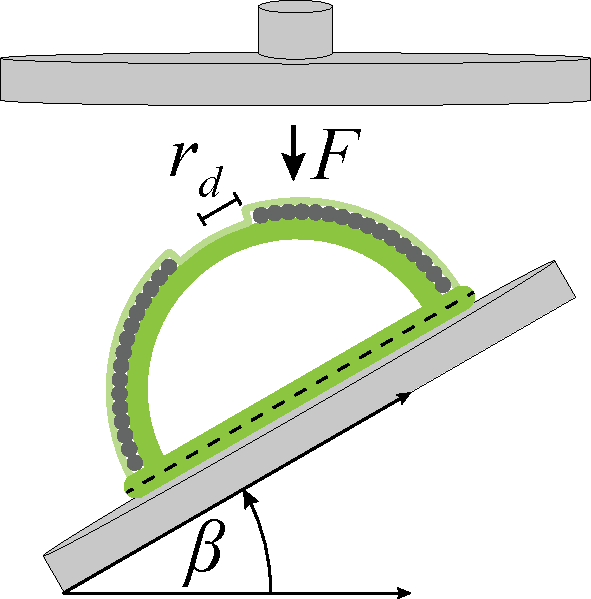
\includegraphics[height=2cm]{IndentationAngle_Diagram}};

			\addlegendentry[scale=0.8]{$r_d=$~4 mm}
			\addlegendentry[scale=0.8]{$r_d=$~6 mm}
			\addlegendentry[scale=0.8]{$r_d=$~8 mm}
			\addlegendentry[scale=0.8]{$r_d=$~10 mm}
			
		\end{axis}
		
	\end{tikzpicture}
	\vspace{1cm}
\end{document}